%%%%% Design %%%%%
\chapter{Figures for Illustration}
\label{append:figures}

\begin{landscape}
    \begin{figure}[H] % figure
        \centering 
        \captionsetup{labelsep=colon}
        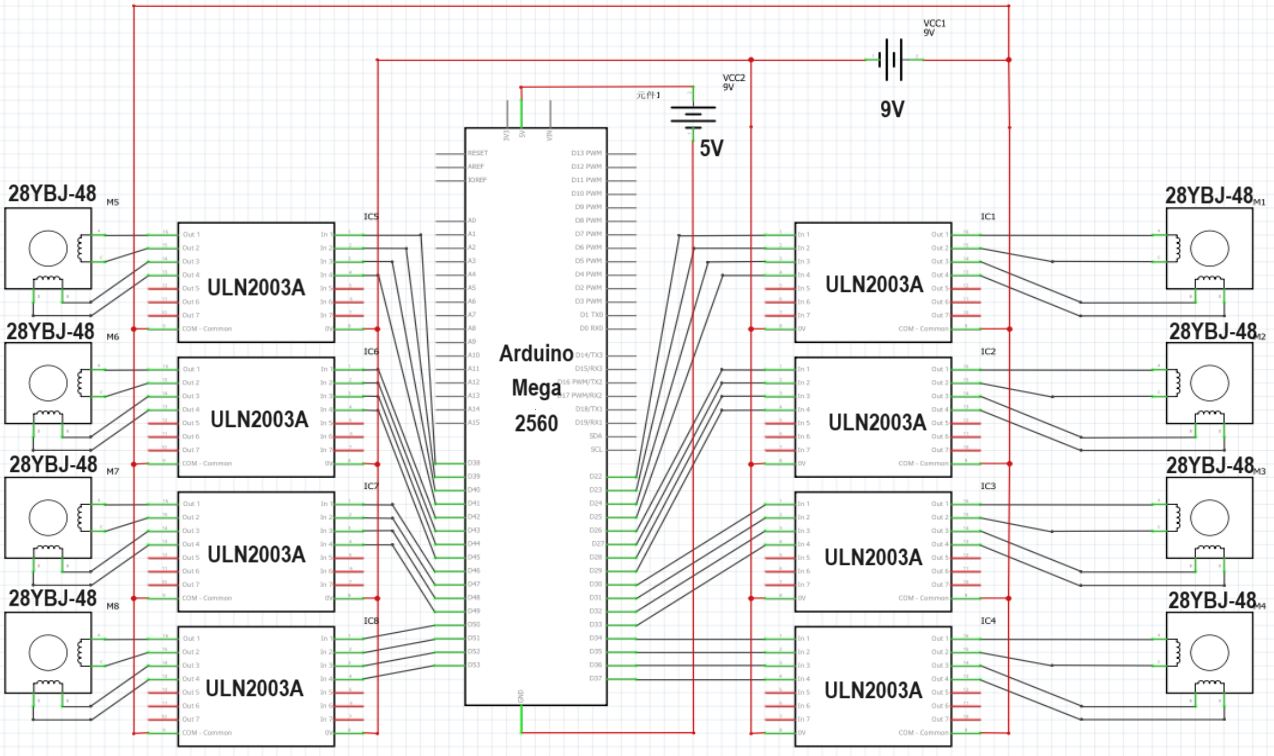
\includegraphics[width=1.5\textwidth]{Image/Design/arduino_circuit_layout.png} 
        \caption[]
        {\centering \textbf{The circuit layout of Arduino step motor control system.}}
        \label{fig:motor_circuit_layout}
    \end{figure}
\end{landscape}
\newpage
\begin{landscape}
    \begin{figure}[H] % figure
        \centering 
        \captionsetup{labelsep=colon}
        \begin{subfigure}{0.62\textwidth} % subfigure 1
            \centering
            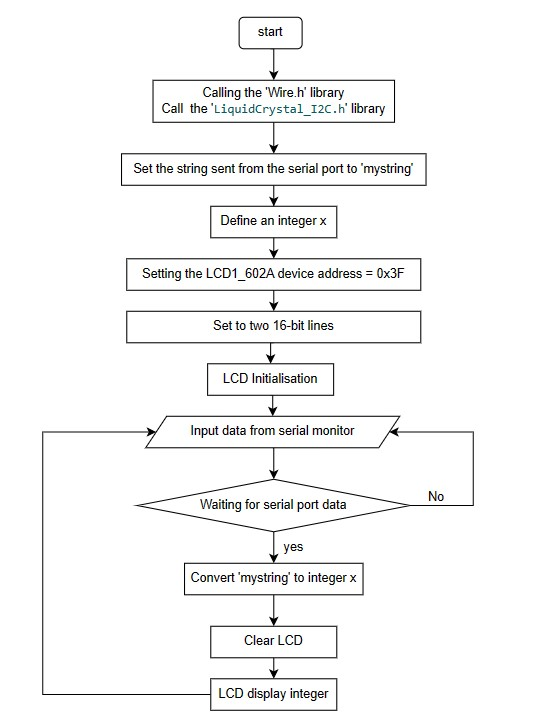
\includegraphics[width=\linewidth]{Image/Design/code_logic_input.jpg}
            \caption{\centering The code logic of using serial \\to input command parameter}
            \label{fig:cl_input}
        \end{subfigure}
        % \hfill
        \begin{subfigure}{0.62\textwidth} % subfigure 2
            \centering
            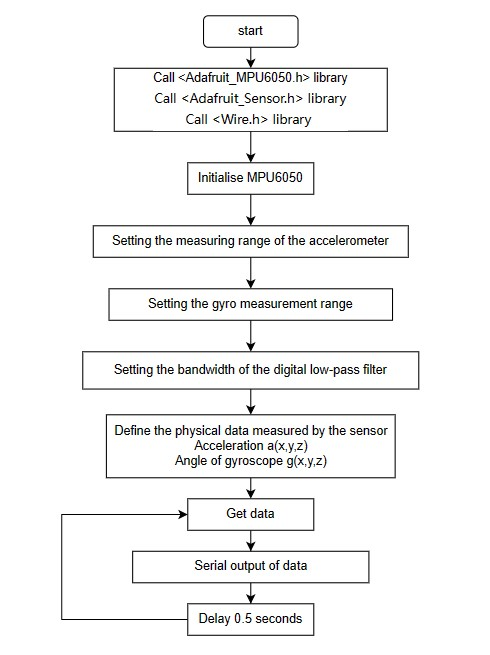
\includegraphics[width=\linewidth]{Image/Design/code_logic_angle.jpg}
            \caption{\centering The code logic of using MPU6050 \\to monitor gyro angles and accelerations}
            \label{fig:cl_angle}
        \end{subfigure}
        \caption[]
        {\centering \textbf{The code logic of input parameters and MPU6050.}}
        \label{fig:cl_input_angle}
    \end{figure}
\end{landscape}
\newpage
\begin{landscape}
    \begin{figure}[H] % figure
        \centering 
        \captionsetup{labelsep=colon}
        \begin{subfigure}{0.715\textwidth} % subfigure 1
            \centering
            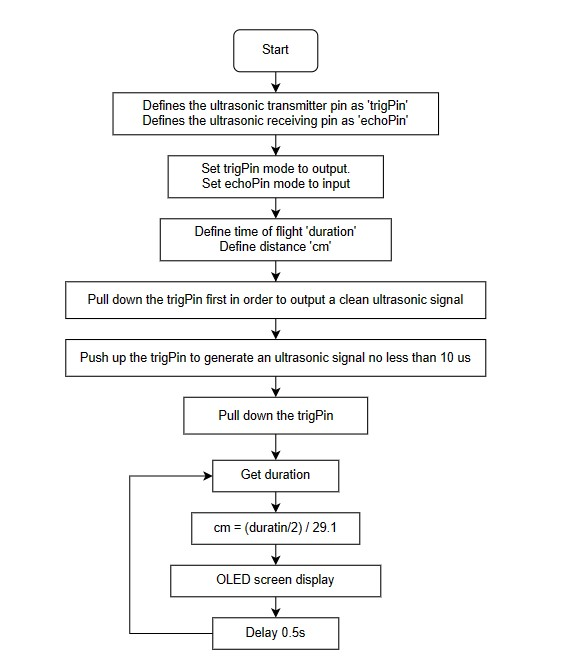
\includegraphics[width=\linewidth]{Image/Design/code_logic_tof.jpg}
            \caption{\centering The code logic of using HC-SR04 \\to measure distance}
            \label{fig:cl_tof}
        \end{subfigure}
        % \hfill
        \begin{subfigure}{0.52\textwidth} % subfigure 2
            \centering
            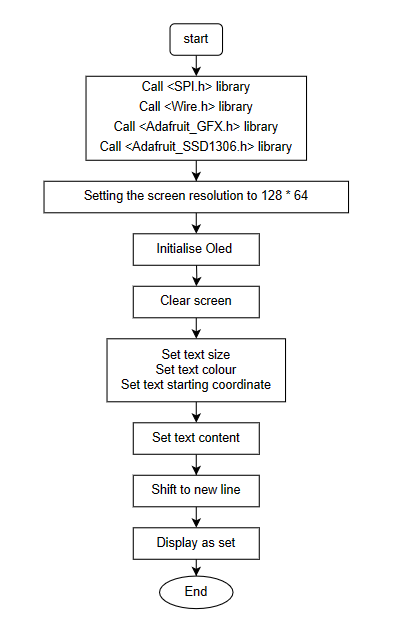
\includegraphics[width=\linewidth]{Image/Design/code_logic_display.png}
            \caption{\centering The code logic of using SSD \\1306 OLED to display data}
            \label{fig:cl_oled}
        \end{subfigure}
        \caption[]
        {\centering \textbf{The code logic of HC-SR04 and SSD 1306 OLED.}}
        \label{fig:cl_tof_oled}
    \end{figure}
\end{landscape}


% change to new page
\newpage